%\documentclass{report}
%\usepackage{fullpage}
%%\usepackage[top=1in, bottom=1in]{geometry}
%\usepackage{amsfonts}
%%for math symbols, Ex: \mathbb{N}
%\def\Definition{what does something mean}
%\usepackage{graphicx}
%\usepackage[hidelinks]{hyperref}
%\usepackage{pdfpages}
%\usepackage{float}
%\usepackage{subcaption}
%
%\begin{document}

\chapter{Methodology}

\section{Setup}

All the experimental data has been collected by Pablo et.al\cite{pablo}. Heated Jet Noise Rig, dual CCD cameras, dual pulse Nd:YAG Laser, 1.0$\mu$ Aluminium Oxide as particle seeds, Olive oil as ambient seed,  C-D conical nozzle of diameters($D_e$) 0.813in,1.085in and design mach number 1.5, 12 equally distributed chevrons with length 0.2D and spacing 0.08D for smaller nozzle have been used for the setup. Each of the four images taken are of resolution 130*170(w*h) with spacing of about 2mm (0.01$D_e$) and then merged to form complete domain. \\

\begin{figure}[H]
\begin{subfigure}{.5\textwidth}
	\centering
	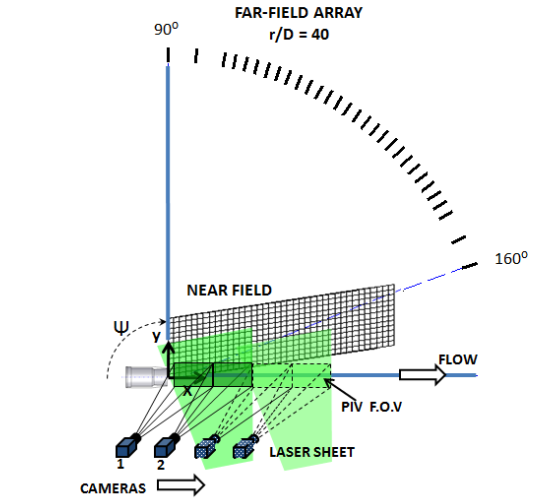
\includegraphics[width=3in]{images/setup.png}
	\caption{Experimental setup}
	\label{fig:setup1}
\end{subfigure}%
\begin{subfigure}{.5\textwidth}
	\centering
	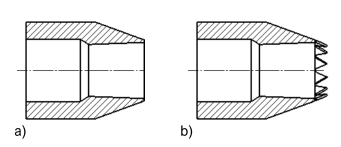
\includegraphics[width=3in]{images/nozzles.png}
	\caption{Nozzles with and without chevrons}
	\label{fig:setup2}
\end{subfigure}
\caption{Nozzles and Experimental setup by Pablo Mora et.al.,}
\label{fig:setup}
\end{figure}

\par\par
Python3.6 has been used to convert experimental column data into array form and create all the plots. Complete code\footnote{ Code and \LaTeX \ files can also be accessed on https://github.com/ravirejo/PIVAnalysis.} is included in the appendix. The only steps to be taken to run the code is to ensure that exit diameter(dia), temperature ratio (NTR) and pressure (NPR) are updated manually in the code (\textit{TRPR }array) and the centre of jet has to be adjusted according to the experimental data. Input files expected are B0001up, B0001Down for \textit{$V_x$}; B0002up, B0002Down for \textit{$V_y$}; B0004up, B0004Down for \textit{TKE} with \_ntr\_npr added to their names where ntr, npr are numerical values in the form of 1p0, 3p6 etc.,

\begin{figure}[H]
\begin{subfigure}{.5\textwidth}
	\centering
	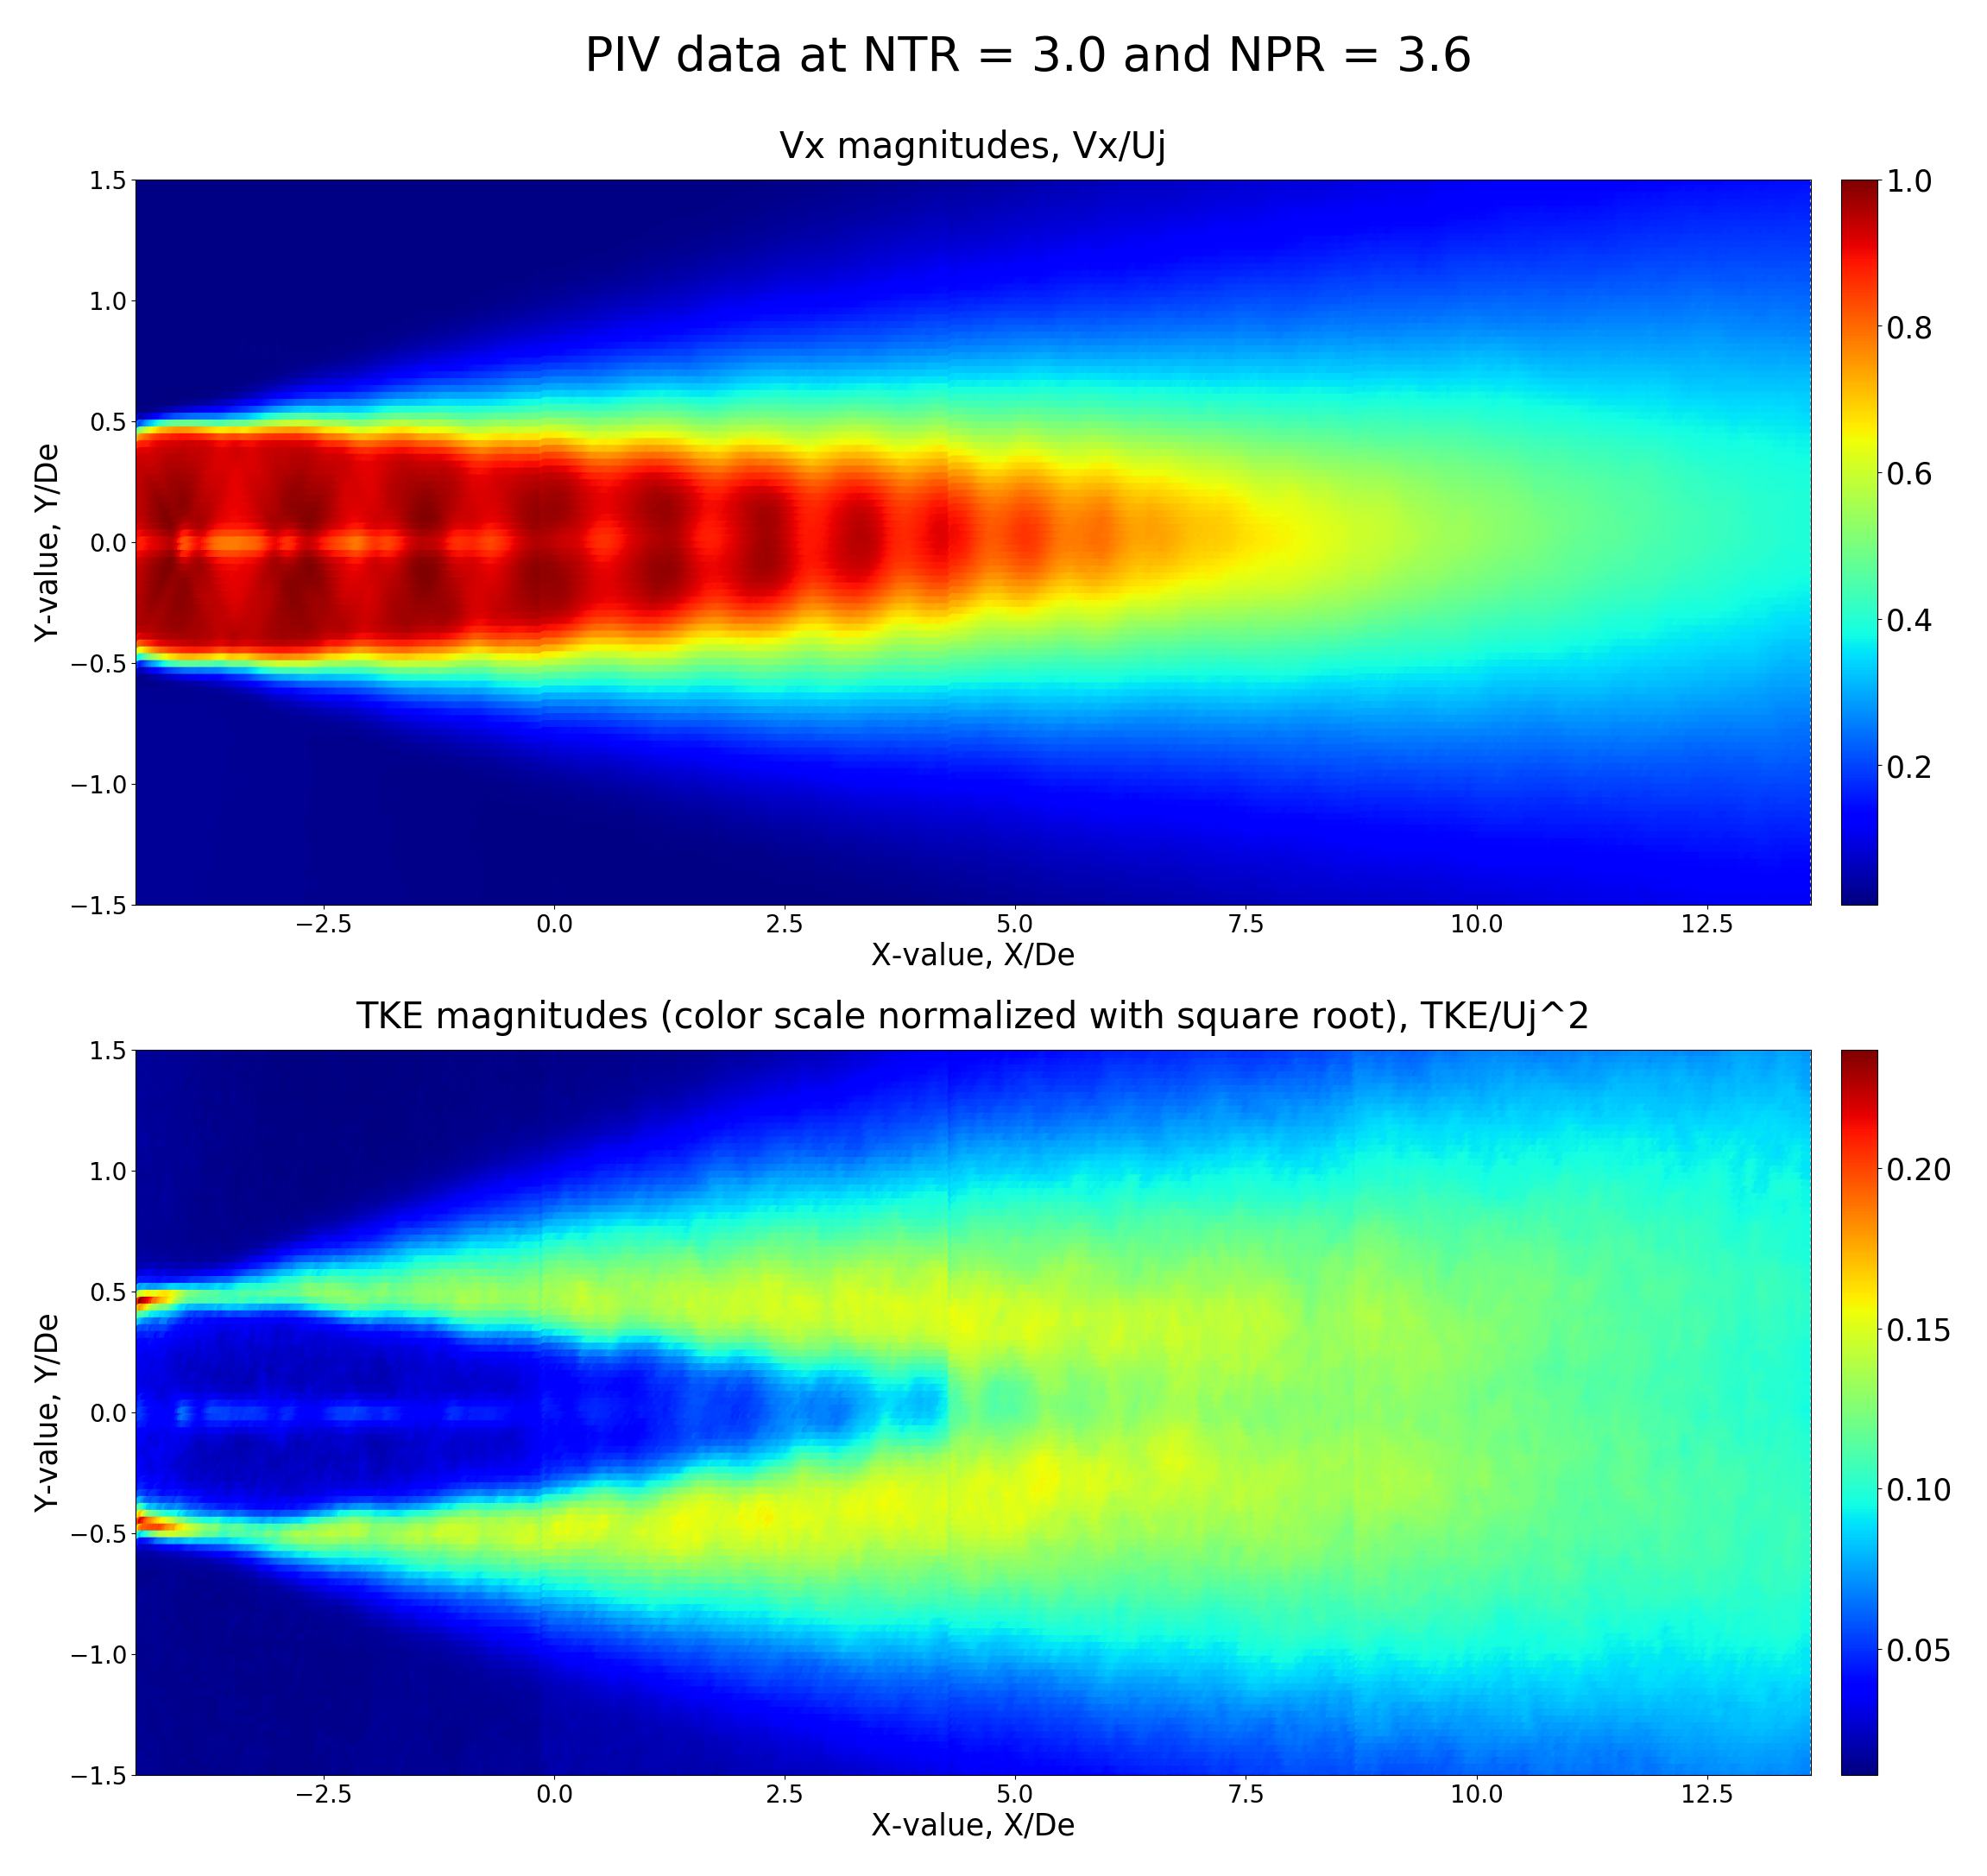
\includegraphics[width=3in]{images/2dsample.png}
	\caption{TKE and Vx at NTR 3.0, NPR 3.6}
	\label{fig:2dsample}
\end{subfigure}%
\begin{subfigure}{.5\textwidth}
	\centering
	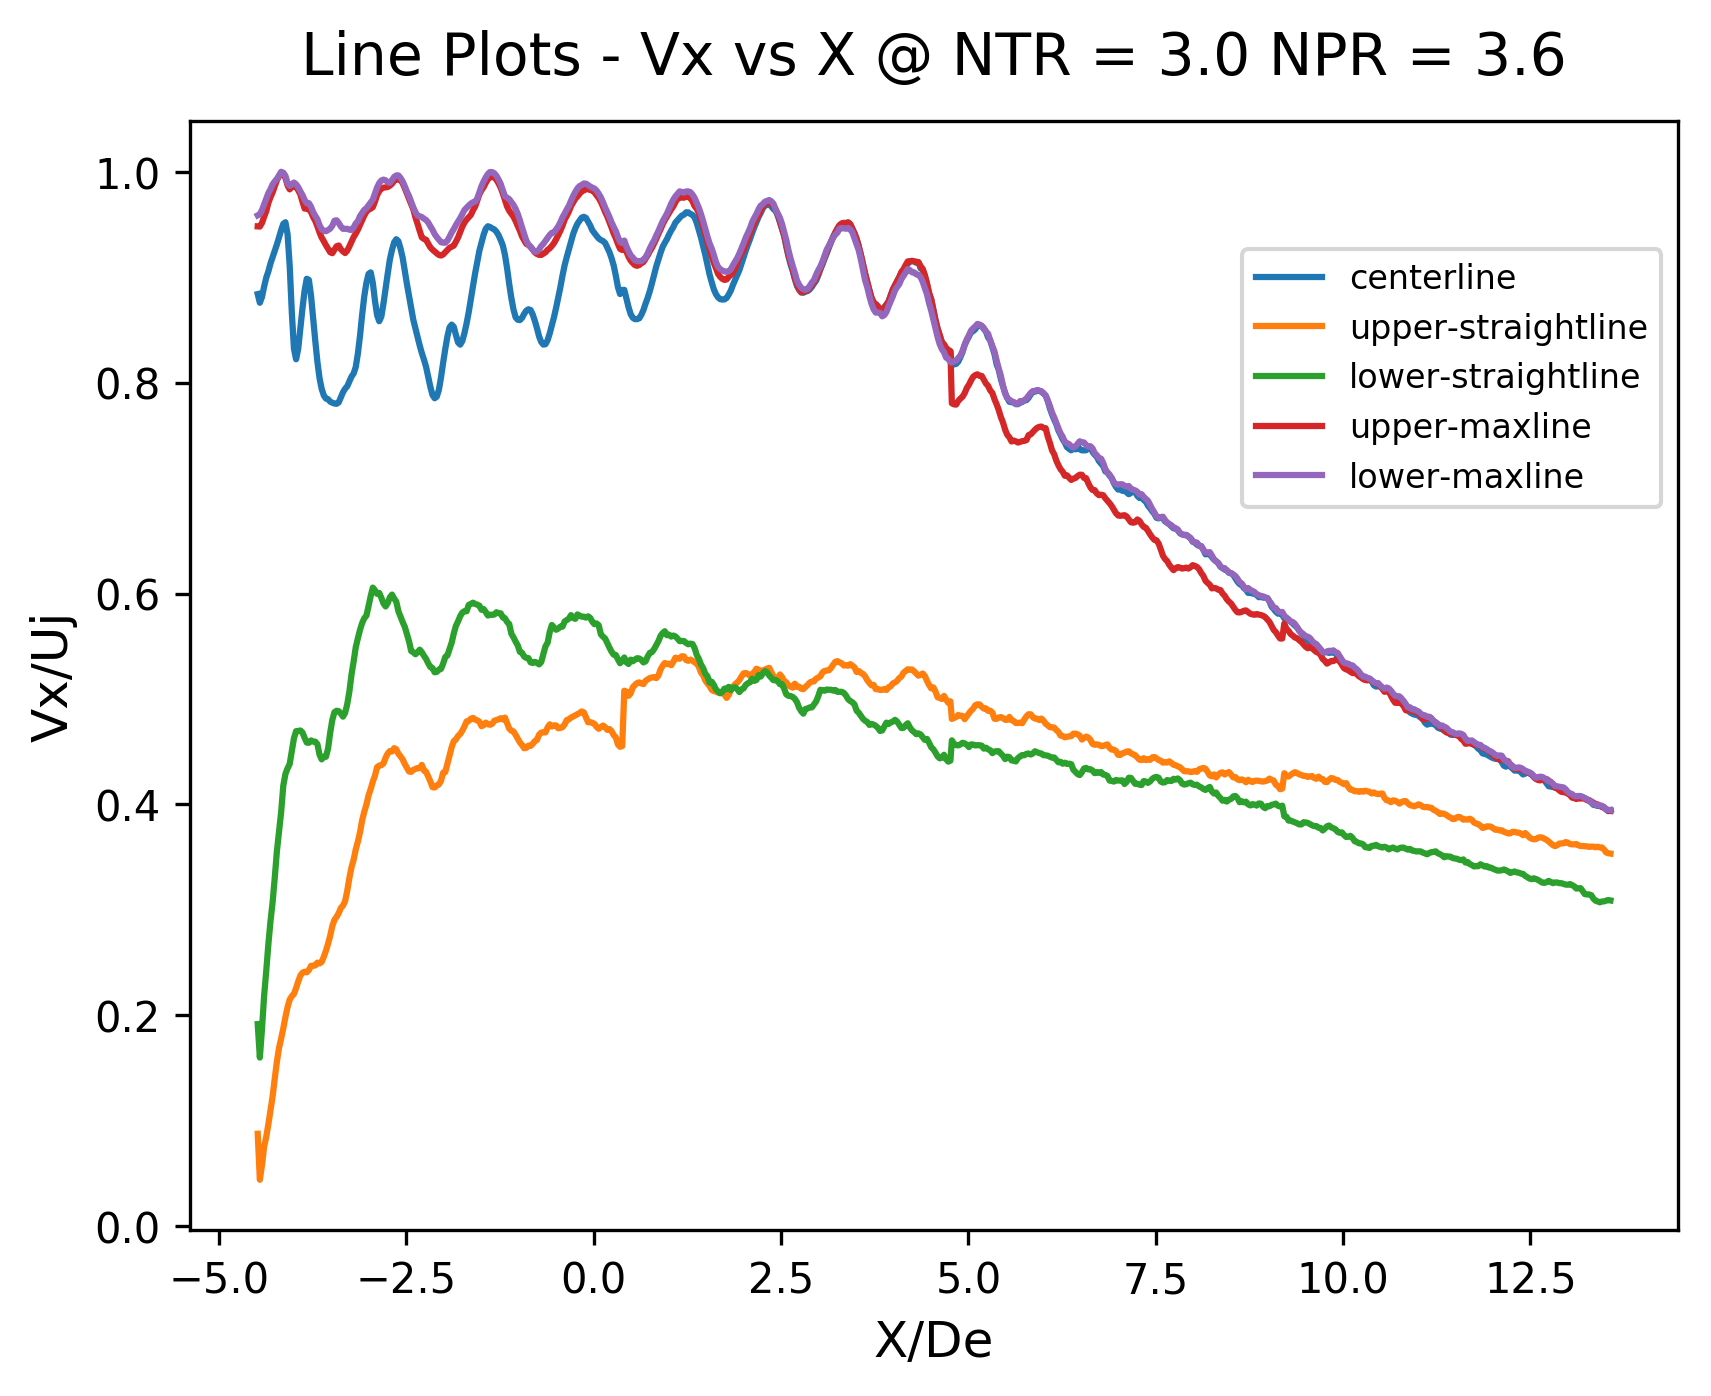
\includegraphics[width=3in]{images/lineplotsample.png}
	\caption{Lineplot of Vx at NTR 3.0, npr 3.6}
	\label{fig:lineplotsample}
\end{subfigure}
\caption{ Domain plot for TKE and Vx, Lineplot for Vx at NTR3.0, NPR3.6.}
\label{fig:2d&lineplot}
\end{figure}

\section{2D image reconstruction}
Data from all the cameras and capture points is merged and contour plots are drawn. Alignment has to be done manually with care since it varies from setup to setup. Both Velocity and Turbulent Kinetic Energy (TKE) (fig \ref{fig:2dsample}) have been normalized with $U_j$ and $U_j^2$ where $U_j$ is jet velocity i.e., max velocity at the exit of nozzle. 

\section{Lineplots}
Lineplots (fig \ref{fig:lineplotsample}) have been drawn for Vx, Vy and TKE for five lines; Centreline is along the centre of jet. Upper and lower straight lines are along the straight lines at lips of jet. Upper and lower maxlines are curves of maximum values above and below centreline. Due to the complexity of experimental setup, exact position of jet centre is not usually at origin and hence has to be accounted manually in the code. But slight discrepancy in vertical position should not be an issue in the present context, since we are more interested in length scales along X.

\begin{figure}[H]
\begin{subfigure}{.5\textwidth}
	\centering
	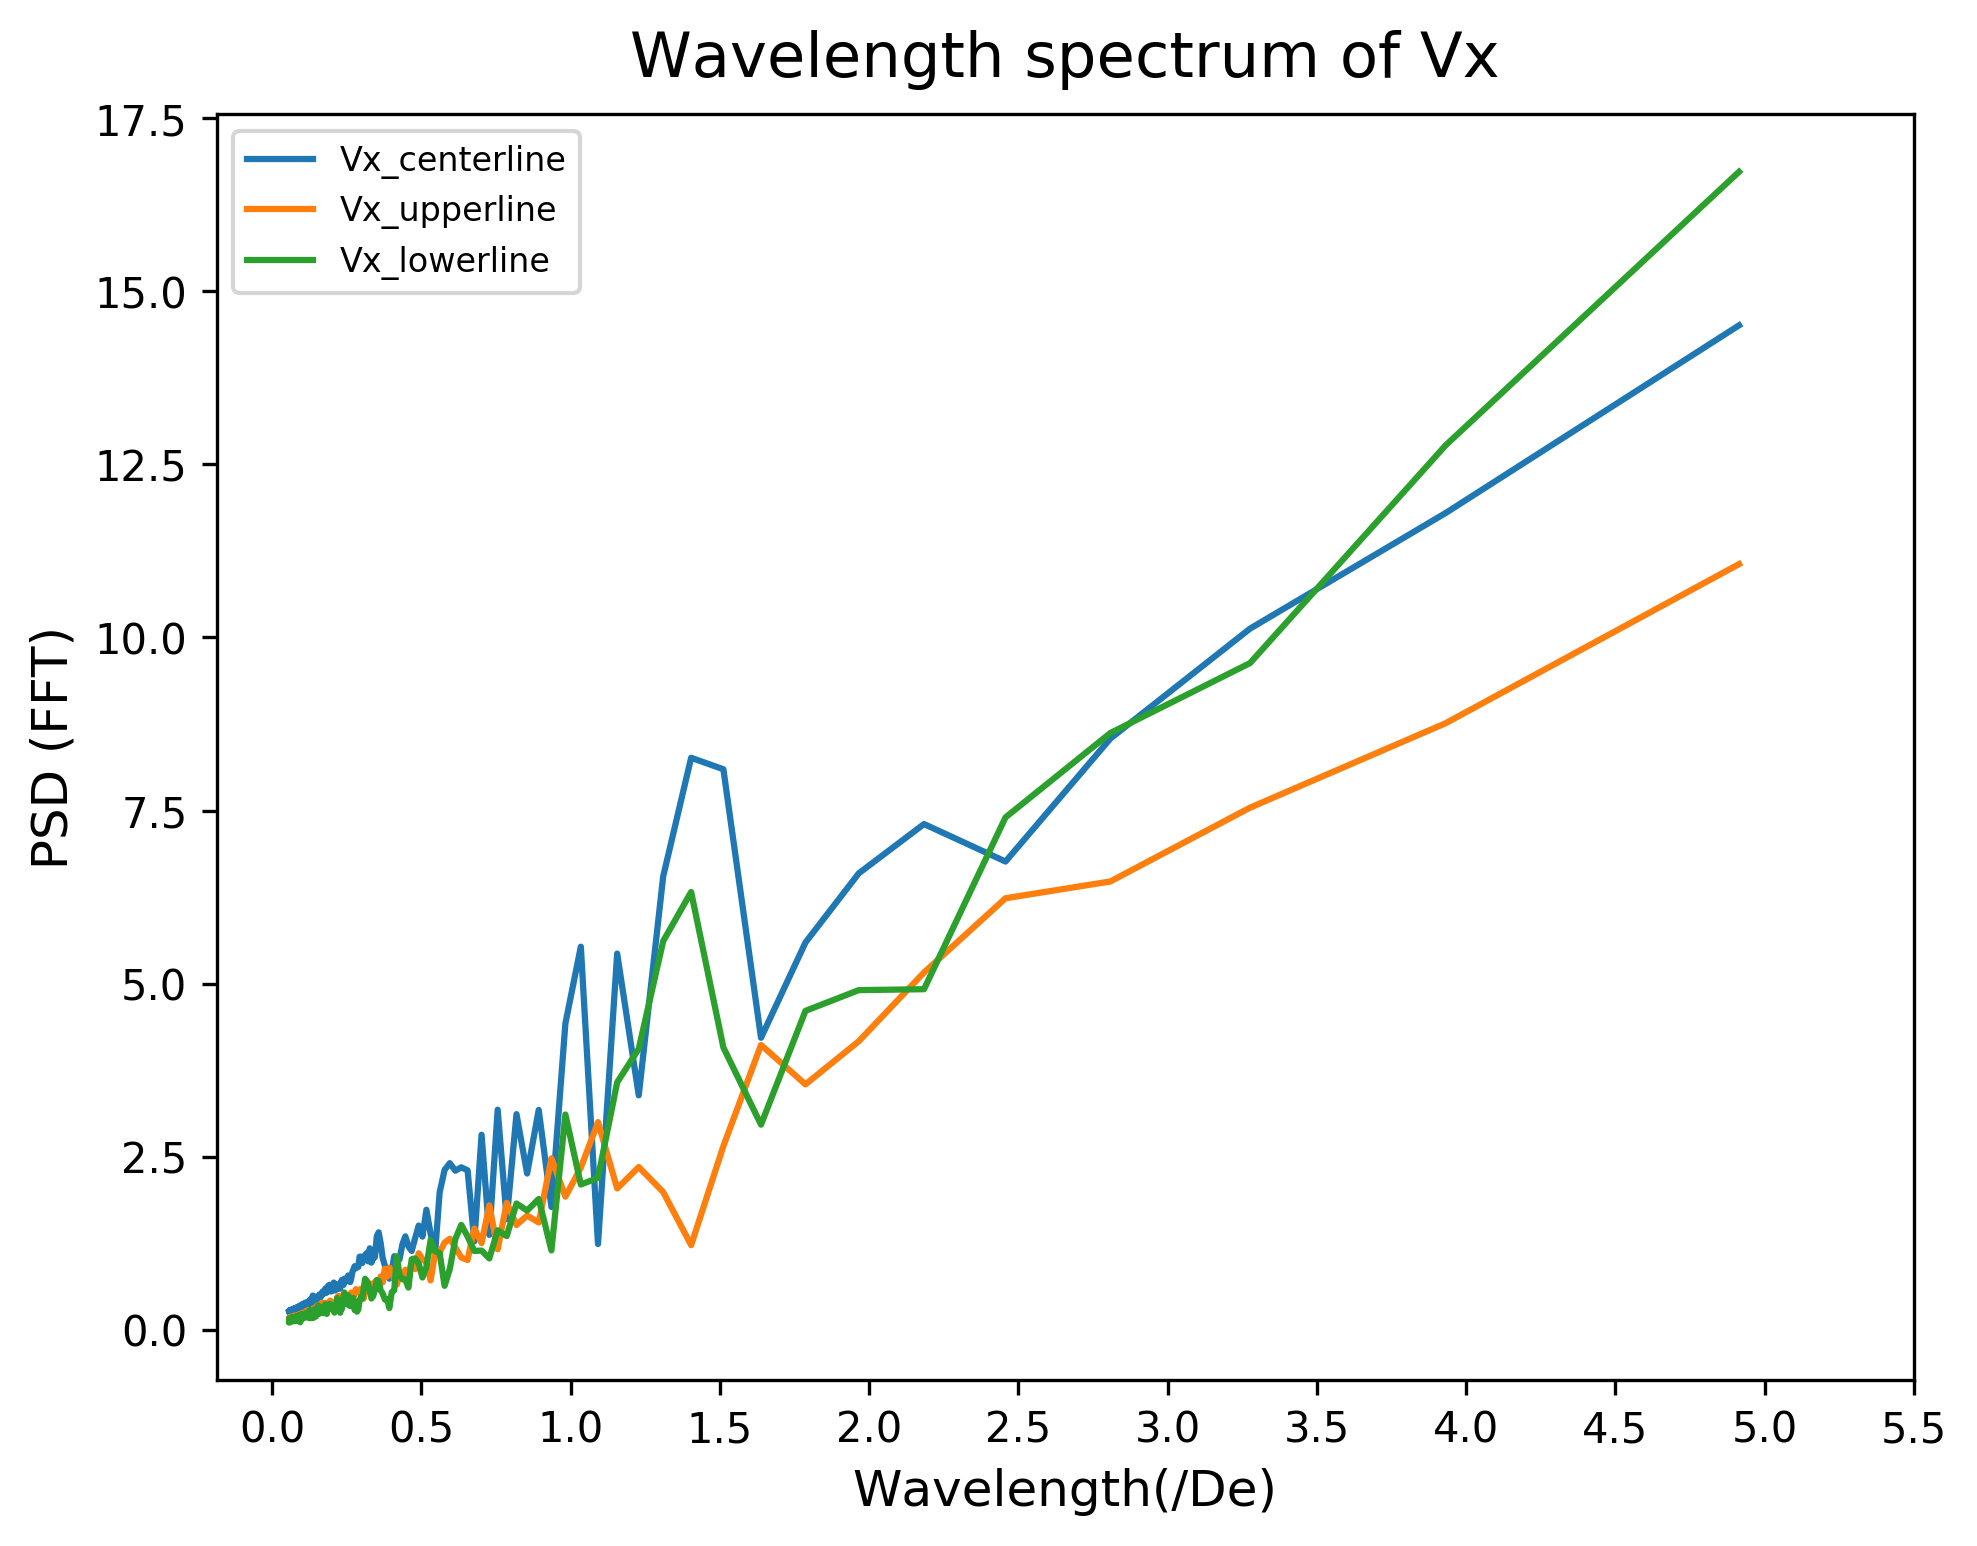
\includegraphics[width=1.5in]{images/fftsample.png}
	\caption{wavelength analysis for Vx at NTR 3.0, NPR 3.6}
	\label{fig:fftsample}
\end{subfigure}%
\begin{subfigure}{.5\textwidth}
	\centering
	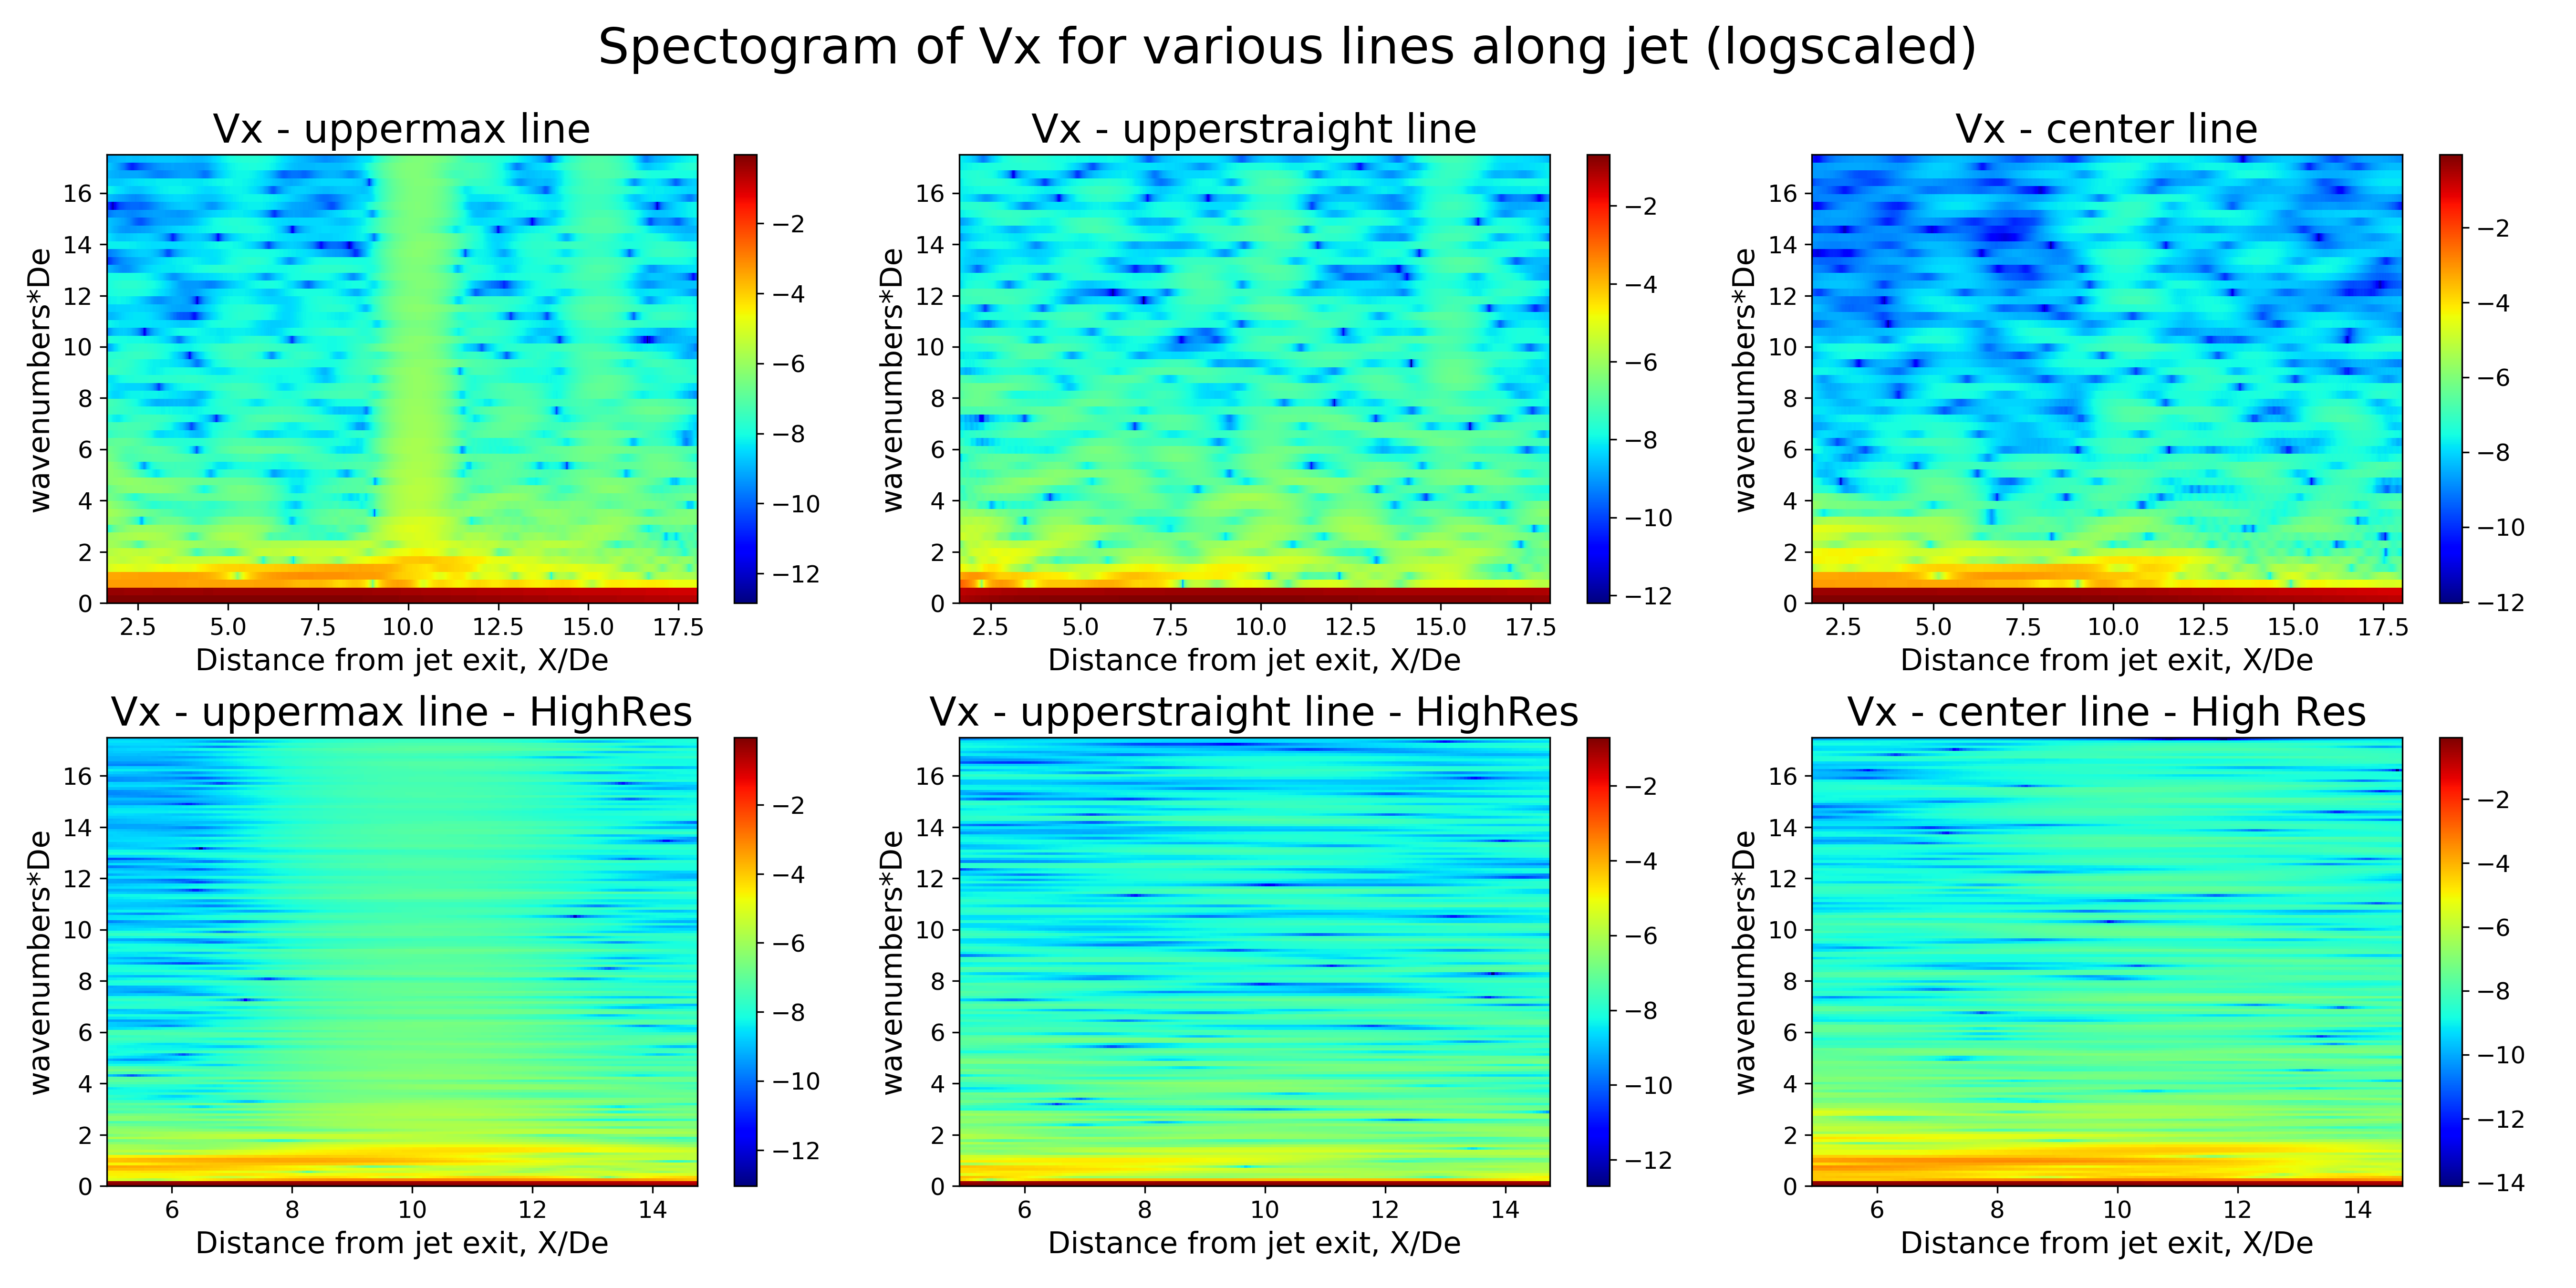
\includegraphics[width=2.5in]{images/spectogramsample.png}
	\caption{Spectogram of TKE at NTR 3.0, npr 3.6}
	\label{fig:spectogramsample}
\end{subfigure}
\caption{ Spectogram for TKE at NTR3.0, NPR3.6.}
\label{fig:fft&spectogram}
\end{figure}

\section{Spatial FFT}
Fast Fourier Transform (FFT) (fig \ref{fig:fftsample}) is a widely used technique to analyse various frequency components in an audio signal. Since we are restricted to steady state analysis for this report, we do not have time data. But we can still apply FFT to the line plot data and obtain velocity scale spectrum ( Power Spectral Density Vs Wavelengths). This can be used to study shock cell lengths and positions with a perspective different from previous methods. FFT has been calculated for three lineplots; centre, upper and lower straightlines. Resolution in x direction is about $1/29^{th}$ of $D_e$. This is taken as sampling rate since we want our wavelength to be normalized by $D_e$ . Linear increase in psd with wavelength could be detrended as we are only interested in the characteristic wavelengths, but has been ignored. We could estimate a rough shock cell length from 2d contour plots but variation along jet length makes it difficult. From FFT, as we can see in fig \ref{fig:fftsample},  it is much easier to quantize the shock cell length distribution.

\section{Spectogram}
FFT is a great tool for component analysis but it does not give information at a specific time instant, or specific position in this context. Spectogram (fig \ref{fig:spectogramsample}) can be used for this purpose. Essentially, spectogram is short FFT taken over a chosen window of fragments of input signal and averaged if fragments are overlapping. So, we have spectrum at centre point of every fragment. Shorter the fragment, higher the resolution in x direction but we have to ensure the fragment is sufficiently longer than length of shock cell to ensure that the relevant wavelength is captured. Higher the overlap between fragments, smoother the transition. Resolution seems to increase in y (wavenumber) direction as observed in \ref{fig:spectogramsample}. But the output to input domain ratio is far less than 1 since the spectogram starts only from the centre of first fragment. Moreover, precision decreases in the direction of x as the signal is smeared because of high overlap. As we can see in fig \ref{fig:spectogramsample}, we know exactly which wavelength is dominating at each of point of jet which is not possible with FFT or difficult to quantize with 2d contour plots.

\section{Shockcell Length}
Shockcell length has been calculated from the analytical equation derived by Tam et.al \cite{tam1}.

\begin{equation}\label{eq:1}
L_s \approx \ \pi \sqrt{(M_j^2-1)} D_j/\mu, \ where \ \mu \ = \ 2.40483
\end{equation}

$D_j$, diameter of jet along the flow, is higher or lower than $D_e$ depending on whether the flow is underexpanded or overexpanded. $M_j$, mach number at the jet centre, generally decreases along the jet as expected. 

%\end{document}